\section{Attested execution: \ArcaneOS, the \SAS, and the attestation network}
\label{sec:attested-execution}\label{sec:attestation}

A node that lies about its own hardware is one problem; a node that boots something other than
the image it claims to run is a different, sharper one. \ArcaneOS is Flux's answer to the second
problem: a hardened Linux image with measured boot, disk encryption tied to the host, and a
signed root filesystem, running a local service (\fluxsas, the \SAS) that other components query
before they trust a node. The chain from firmware to a locked-down running system does real,
verifiable work, and the update mechanism that ships new images is a carefully engineered,
deliberately centralized ceremony. What the resulting \emph{attestation} — the signed statement a
node can produce about itself — does not do is bind that statement to the specific machine that
produced it. This section describes the deployed chain first, states exactly where that binding
fails, and then specifies the bonded attestation network the roadmap proposes as the fix: an
approach that replaces "trust the key" with "trust the capital at risk," which is a primitive
Flux already has and a hardware root of trust is not.

\subsection{The deployed attestation stack}

\subsubsection{The boot chain}
\label{sec:boot-chain}

On a bare-metal or VPS install, \ArcaneOS's Secure Boot Platform Key (PK), Key Exchange Key (KEK)
and signature database (db) are written into the machine's live UEFI variables at install time
from \texttt{.auth} artifacts staged on the EFI system partition, replacing whatever keys were
present, after which the revocation database (dbx) is made immutable with \texttt{chattr~+i}
\shipped~\srccode{fluxos-iso/\allowbreak{}flux\_fs/\allowbreak{}fs\_scaffold/\allowbreak{}curtin/\allowbreak{}curtin-hooks}{26--43}. This is a
Flux-controlled Platform Key, not a hardware-vendor or Microsoft key: its SHA-256 hash is a
build-time constant (\texttt{FLUX\_PK\_SHA256SUM}) baked into the \texttt{fes} ("Flux Enrollment
Service") binary \shipped~\srccode{fluxos-iso/\allowbreak{}Makefile}{65}.

At boot, \texttt{fes} and \fluxsas independently re-derive that trust. \fluxsas's
\texttt{check\allowbreak{}Secure\allowbreak{}Boot()} reads the UEFI \texttt{SecureBoot} variable and calls a fatal
\texttt{terminateApp()} if Secure Boot is not enabled \shipped~\srccode{fluxsas/\allowbreak{}src/\allowbreak{}sas.cpp}{101--110}.
\texttt{fes} performs the identical check during first-boot enrollment and, on the initrd side,
\texttt{fes-wrapper} treats \texttt{fes}'s exit code as its entire contract: exit \texttt{50}
means Secure Boot is disabled, \texttt{51} means the enrolled Platform Key's hash did not match
the pinned value, \texttt{52} means no TPM2 device is present, and any other nonzero code is a
generic enrollment failure — on any of these, the initrd prints a warning to the console, waits
up to 30~seconds, and powers the machine off rather than continuing to boot
\shipped~\srccode{fluxos-iso-pkcs11/\allowbreak{}99flux-crypt/\allowbreak{}fes-wrapper}{1--45}. The fuller code set
(\texttt{53}--\texttt{57}, covering TPM2 enrollment failure, the VPS check, PKCS\#11 enrollment,
keystore failure and device-unlock failure) is defined alongside these in the same enrollment
tool \shipped~\srccode{fluxsas/\allowbreak{}secrets}{FES\_EXIT\_* block}. This is a real fail-closed boot gate,
correctly credited: a node that cannot prove Secure Boot is on, with the right key, and a TPM2
present, does not come up at all.

Where a TPM2 device exists, \texttt{fes} enrolls it against the system LVM volume with
\texttt{systemd-\allowbreak{}cryptenroll -\allowbreak{}-\allowbreak{}wipe-\allowbreak{}slot=all -\allowbreak{}-\allowbreak{}tpm2-\allowbreak{}device=auto -\allowbreak{}-\allowbreak{}tpm2-\allowbreak{}pcrs=7}
\shipped~\srccode{fluxsas/\allowbreak{}src/\allowbreak{}fes/\allowbreak{}fes.cpp}{173--186}. Only PCR~7 is sealed against — the PCR that
measures Secure Boot policy state (PK/KEK/db/dbx contents and the enabled flag), not the kernel,
initrd, or root filesystem image. The direct consequence, read from the enrollment code rather
than inferred, is that a TPM-sealed key unseals for \emph{any} kernel and initrd signed under the
pinned Platform Key, not specifically the build that was running when the key was sealed —
image-version binding is not something the TPM seal itself provides.

Root disk unlock is offered both hardware and software paths simultaneously:
\texttt{systemd-cryptsetup@root.\allowbreak{}service} attaches the root LUKS volume with
\texttt{tpm2-\allowbreak{}device=auto,pkcs11-\allowbreak{}uri=auto} set together
\shipped~\srccode{fluxos-iso-pkcs11/\allowbreak{}99flux-crypt/\allowbreak{}cryptsetup-wrapper}{5--7}. Where no TPM2 device
is present, \texttt{fes} first checks whether the host is a hosting/VPS IP via a third-party
lookup \shipped~\srccode{fluxsas/\allowbreak{}src/\allowbreak{}fes/\allowbreak{}fes.cpp}{205--236}, then falls back to a software PKCS\#11
token: an RSA-4096 key generated inside a SoftHSM2 store held in an encrypted loopback image
\shipped~\srccode{fluxsas/\allowbreak{}src/\allowbreak{}fes/\allowbreak{}fes.cpp}{102--141,244--276}, with a PIN derived from local machine values
and written in plaintext to \texttt{/\allowbreak{}etc/\allowbreak{}credstore/\allowbreak{}cryptsetup.\allowbreak{}pkcs11-pin} — a placement the source
comment itself flags as unresolved (\emph{"Move this to socket"})
\shipped~\srccode{fluxsas/\allowbreak{}src/\allowbreak{}fes/\allowbreak{}fes.cpp}{239--241,356}. \textbf{This fallback is where the
guarantee weakens}: the SoftHSM2 token database is protected at rest by a static key compiled into
every \fluxsas binary rather than by hardware, so per-machine sealing degrades to
per-machine-plus-anyone-who-reads-the-binary sealing. The fallback exists mainly for VPS hosts
that do not expose custom Secure Boot key enrollment to the guest, and the \ArcaneOS documentation
itself notes this population is shrinking as providers close that off
\srcdoc{fluxos-iso/README.md:289--296}.

Root filesystem integrity is enforced by dm-verity: \fluxsas parses \texttt{veritysetup status}
for the active root hash and its \texttt{verified} status
\shipped~\srccode{fluxsas/\allowbreak{}src/\allowbreak{}watchdog.h}{449--506}. This confirms the running rootfs is mounted
under dm-verity; the boot-time source of the \emph{expected} root hash consumed by the initrd is
not established by the evidence available for this section and is not asserted here. Finally, the
initrd mitigates the physical-access window between an unattended install and first boot: once a
disk-unlock token has been enrolled, \texttt{flux-\allowbreak{}init-\allowbreak{}cleanup} mounts the plaintext,
\texttt{root}-labelled filesystem and deletes everything on it except the current squashfs image,
its verity file, install logs, and small configuration files, specifically "to mitigate the
primary drive being mounted by an attacker after installation, but before first boot"
\shipped~\srccode{fluxos-iso-pkcs11/\allowbreak{}99flux-crypt/\allowbreak{}flux-init-cleanup}{20--60}. A real window remains
between install completion and that cleanup pass, during which the plaintext root and the
unencrypted EFI system partition are both mountable by anyone with physical access to the disk.

\subsubsection{The update channel}
\label{sec:update-channel}

The strongest link in the chain is how a new \ArcaneOS image reaches every node. Release signing
runs through a physically Flux-operated YubiHSM~2, whose objects include a dedicated Ed25519
release-signing key (\texttt{Flux\allowbreak{}Os\allowbreak{}Release\allowbreak{}Key}) alongside the Secure Boot signing keys
\shipped~\srccode{flux-iso-hsm/\allowbreak{}src/\allowbreak{}flux\_hsm/\allowbreak{}hsm\_manager.py}{178--544}. A human custodian
authenticates to the HSM with their own personal YubiKey via challenge-response key derivation, so
no raw password ever leaves the YubiKey \shipped~\srccode{flux-iso-hsm/\allowbreak{}src/\allowbreak{}flux\_hsm/\allowbreak{}hsm\_manager.py}{686--764},
and a build session's actual signing credentials are fresh, single-use authentication keys created
for that session and expected to be deleted afterward
\shipped~\srccode{flux-iso-hsm/\allowbreak{}src/\allowbreak{}flux\_hsm/\allowbreak{}hsm\_manager.py}{1064--1110}. The HSM's own master
wrap key is backed up by Shamir's Secret Sharing across an $M$-of-$N$ set of custodians, driven end
to end over a dedicated ceremony protocol
\shipped~\srccode{flux-iso-hsm/\allowbreak{}src/\allowbreak{}flux\_hsm/\allowbreak{}server/\allowbreak{}sss.py}{12--37}. A finished build is bundled
into a release tarball and signed with that Ed25519 key over a chunked SHA-256 digest of the whole
artifact \shipped~\srccode{fluxos-iso/\allowbreak{}flux-release-signer/\allowbreak{}src/\allowbreak{}flux\_release\_signer/\allowbreak{}main.py}{69--152};
every node verifies incoming updates against a single Ed25519 public key baked into the image at
build time \shipped~\srccode{fluxos-iso/\allowbreak{}flux\_fs/\allowbreak{}build\_target.sh}{81--84}.

Stated plainly: \textbf{only Flux can publish an \ArcaneOS update.} Every node verifies an incoming
update against exactly one embedded Ed25519 public key and no other
\shipped~\srccode{fluxos-iso/\allowbreak{}flux\_fs/\allowbreak{}build\_target.sh}{81--84}, and the only private key that
verifies against it lives inside the Flux-operated HSM behind the custodian ceremony described
above \shipped~\srccode{flux-iso-hsm/\allowbreak{}src/\allowbreak{}flux\_hsm/\allowbreak{}hsm\_manager.py}{336,1064--1110}; whoever holds
that HSM key can therefore produce an update every node's updater will accept. This is not an
oversight; the ceremony design — personal-YubiKey custodian authentication, single-use per-build
signing keys, and Shamir-split master-key recovery, all cited above — is a deliberate, carefully
engineered centralization of exactly one function. It should be read as such rather than
apologized for. (A WireGuard-tunneled fast path for the signing session exists alongside the
default SSH-tunneled one but is gated behind a flag documented as defaulting to off, and is tagged
\inprogress here rather than folded into the ceremony's shipped description
\srcdoc{flux-iso-hsm/docs/SETUP\_FLOW.md:333--353}.) The
one caveat worth stating alongside it: the same build scripts that produce production releases
also carry explicit debug bypasses (\texttt{SKIP\_RELEASE\_SIGNING}, \texttt{SKIP\_LIVE\_SIGNING})
that ship an unsigned tarball, UKI, or kernel module if set
\shipped~\srccode{fluxos-iso/\allowbreak{}build\_dist.sh}{101--114}
\srccode{fluxos-iso/\allowbreak{}flux\_fs/\allowbreak{}build\_kmss.sh}{50--53}
\srccode{fluxos-iso/\allowbreak{}live\_iso/\allowbreak{}build\_uki.sh}{47--48}; if either flag is set on a production
build, the signature chain for that artifact is void, and no code in these repositories checks
that a released artifact was actually signed before publication.

\subsubsection{The \fluxsas protocol}

\fluxsas serves a single listener at \texttt{https:/\allowbreak{}/\allowbreak{}127.\allowbreak{}0.\allowbreak{}0.\allowbreak{}1:16100}, bound to loopback, with
mutual TLS mandatory (\texttt{SSL\_VERIFY\_PEER\allowbreak\;|\;SSL\_VERIFY\_FAIL\_IF\_NO\_PEER\_CERT})
\shipped~\srccode{fluxsas/\allowbreak{}src/\allowbreak{}api\_server.h}{1042--1053,1020}. Authorization beyond the TLS
handshake is by client-certificate Common Name, checked once in a routing handler with no
per-route pinning at the TLS layer itself: the CN \fluxbench is authorized for every route
without exception, the CN \texttt{fdm-nginx} is authorized only for three routes
(\texttt{/v2/decrypt}, \texttt{/\allowbreak{}v2/\allowbreak{}ca\allowbreak{}Certificate}, \texttt{/v2/health}), and any other or missing
CN is rejected with HTTP~403 \shipped~\srccode{fluxsas/\allowbreak{}src/\allowbreak{}api\_server.h}{220--252}. Both
authorized callers are Flux-operated, node-local processes, not tenant-facing ones — a fact with
consequences below. Because \fluxbench carries blanket access, compromising it is
equivalent to compromising everything \fluxsas can sign, encrypt, or decrypt on that host, and
\fluxbench's own mTLS client identity toward \fluxsas is a hardcoded, network-wide Ed25519
keypair shipped in \fluxbench's source, not a per-node credential
\shipped~\srccode{fluxbench/\allowbreak{}src/\allowbreak{}fluxnode/\allowbreak{}sasclient.h}{73--99,80--84}.
The two checkouts read for this subsection do not interoperate: \fluxbench (\texttt{5504e5c},
2026-05-29) probes a plain-HTTP \texttt{localhost:\allowbreak{}16100} and sends its mTLS requests to
\texttt{https:/\allowbreak{}/\allowbreak{}localhost:16102}
\srccode{fluxbench/\allowbreak{}src/\allowbreak{}fluxnode/\allowbreak{}benchmarks.cpp}{4106}
\srccode{fluxbench/\allowbreak{}src/\allowbreak{}fluxnode/\allowbreak{}sasclient.h}{161,166}, while \fluxsas
(\texttt{711776d}, 2026-08-27) serves mTLS only, on 16100, and has no listener on 16102
\srccode{fluxsas/\allowbreak{}src/\allowbreak{}api\_server.h}{972--973,1046--1048}.
\notestablished{which \fluxbench and \fluxsas versions are paired on deployed nodes; the checkouts
read here are three months apart and incompatible as read, so the client behaviour in this
subsection is \fluxbench's and the listener behaviour is \fluxsas's, each at its own checkout.}

The route family of interest for attested execution is \texttt{/v2/attest} (Ed25519-signs a
caller-supplied message under a domain-separated key selected by a \texttt{purpose} argument —
absent, \texttt{cdn}, \texttt{mesh}, or \texttt{app}) and \texttt{/\allowbreak{}v2/\allowbreak{}attestationPublicKey} (returns
the corresponding public key) \shipped~\srccode{fluxsas/\allowbreak{}src/\allowbreak{}api\_server.h}{412--481,483--517}.
Adjacent routes cover a per-app transport key with its own domain-separated attestation
\shipped~\srccode{fluxsas/\allowbreak{}src/\allowbreak{}api\_server.h}{582--653} and a blob-upload signer
\shipped~\srccode{fluxsas/\allowbreak{}src/\allowbreak{}api\_server.h}{750--829}. Freshness is enforced unevenly: only the
\texttt{upload} and \texttt{manifest} kinds of \texttt{/\allowbreak{}v2/\allowbreak{}sign\allowbreak{}Blob\allowbreak{}Upload} check a $\pm300$-second
timestamp window at signing time \shipped~\srccode{fluxsas/\allowbreak{}src/\allowbreak{}api\_server.h}{183,780--829};
\texttt{/v2/attest} and \texttt{/\allowbreak{}v2/\allowbreak{}transportPublicKey} carry no server-enforced freshness at all,
so a verifier consuming either must supply its own staleness policy.

What a verifier learns from a successful \texttt{/v2/attest} call under \texttt{purpose=app} — the
route intended to bind a stored content hash to a validated envelope hash — is that some running
\fluxsas process produced a valid signature over that pair. Whether that constitutes evidence about
\emph{which} host produced it, and under what boot state, is exactly the question the next two
subsections answer.

\subsubsection{The trust root}

\begin{assumption}[The deployed attestation trust root]
\label{asm:trust-root}
The statement "this node booted something Flux considers legitimate" rests today on a compound
root that is entirely Flux-operated:
\begin{enumerate}
  \item a Flux-controlled UEFI Secure Boot Platform Key, pinned by hash inside the \texttt{fes}
  binary and checked against whatever key the firmware has enrolled
  \shipped~\srccode{fluxsas/\allowbreak{}src/\allowbreak{}fes/\allowbreak{}fes.cpp}{70--81};
  \item a Flux-operated pair of web services (\texttt{stats.\allowbreak{}runonflux.\allowbreak{}io} and
  \texttt{arcanehashes.\allowbreak{}app.\allowbreak{}runonflux.\allowbreak{}io}) that publish the set of dm-verity root hashes a node's
  watchdog treats as known-good, polled roughly once every 24--48 hours
  \shipped~\srccode{fluxsas/\allowbreak{}src/\allowbreak{}watchdog.h}{721--754}, and which \textbf{fail open}: if both
  endpoints are unreachable, the watchdog treats the running node as secure and takes no action
  \shipped~\srccode{fluxsas/\allowbreak{}src/\allowbreak{}watchdog.h}{566--596}; and
  \item a Flux-operated internal mTLS certificate authority that issues the client and server
  certificates every \fluxsas caller and listener presents.
\end{enumerate}
No independent hardware vendor, third-party attestation authority, or externally verified TPM
quote appears anywhere in this root.
\end{assumption}

None of this makes the boot chain worthless: measured boot, dm-verity, and LUKS unlock all impose
real, verifiable cost on a remote attacker with no local access. It does mean the assurance a node
offers is a Flux-operated one, not a hardware-rooted, independently verifiable one, and later
claims in this paper build on Assumption~\ref{asm:trust-root} exactly as stated, not on a stronger
reading of it.

\subsubsection{The property that does not hold}

\begin{property}[Attestation is not machine-bound]
\label{prop:not-machine-bound}
The Ed25519 signing key \texttt{/v2/attest} uses for the default, \texttt{cdn}, \texttt{mesh}, and
\texttt{app} purposes is derived by a key-derivation function from static values compiled
identically into every \fluxsas binary; none of the derivation's inputs depends on the TPM, on
Secure Boot state, or on any other per-machine value
\shipped~\srccode{fluxsas/\allowbreak{}src/\allowbreak{}api\_server.h}{411--481,466--469,503--506}. The one exception, the
node-identity key pair (\texttt{/\allowbreak{}v2/\allowbreak{}nodeIdentityPublicKey}, \texttt{/\allowbreak{}v2/\allowbreak{}nodeIdentitySign}), does
mix in a value derived from local machine identifiers, but the key that protects the random
component of that value at rest is itself a static value compiled into every binary
\shipped~\srccode{fluxsas/\allowbreak{}src/\allowbreak{}disk\_encryption.h}{200--228}. Consequently, a valid \fluxsas
attestation demonstrates possession of something every copy of the software contains — it does
not demonstrate that a particular machine booted a particular image. Compile-time obfuscation of
these constants changes what a casual binary scan reveals; it does not change this property.
\end{property}

This is stated as a property that fails, not as a procedure: no derivation input, salt, domain
value, or extraction path appears above or anywhere in this section, and none is needed to state
the property precisely. Property~\ref{prop:not-machine-bound} is the reason the bonded network
described in \S\ref{sec:bonded-network} exists, and it is the reason its Requirement~0 is written
the way it is.

\subsubsection{What a tenant can verify}
\label{sec:tenant-verify}

Today, nothing. Every \texttt{/v2/*} route on \fluxsas requires a client certificate issued by the
internal Flux mTLS CA and is reachable only on loopback
\shipped~\srccode{fluxsas/\allowbreak{}src/\allowbreak{}api\_server.h}{1042--1053,220--252}; an external tenant deploying an
application onto a \FluxOS node has no network path to \fluxsas at all, mTLS or otherwise. The
closest thing to a tenant-visible signal is the \texttt{purpose=app} attestation described above,
and no code path in the read repositories surfaces that signature to a tenant. Even if one did,
per Property~\ref{prop:not-machine-bound} it would prove "some \fluxsas process signed this," not
"this specific host booted a known-good image." There is no tenant-facing verification API, no
TPM-quote endpoint, and no remote-attestation client anywhere in \fluxsas or its provisioning
tooling.

\subsubsection{Residual trust surface}

Beyond the trust root of Assumption~\ref{asm:trust-root}, the deployed system asks a tenant to
accept the following, none of which \fluxsas measures or attests to:
\begin{itemize}
  \item \textbf{The container runtime.} Nothing in \fluxsas measures the Docker or Podman daemon;
  \texttt{are\allowbreak{}All\allowbreak{}Services\allowbreak{}Inactive()} checks that \texttt{containerd}, \texttt{docker.service}, and
  related units are \emph{inactive} before an unmount, which is a shutdown gate, not an integrity
  check \shipped~\srccode{fluxsas/\allowbreak{}src/\allowbreak{}disk\_encryption.h}{547--559,642}.
  \item \textbf{\FluxOS itself.} Application orchestration code runs outside \fluxsas's scope
  entirely; no file in the read evidence measures or attests to it.
  \item \textbf{Physical access.} Console access is explicitly exempted from the password-hash
  check applied to every other local account \shipped~\srccode{fluxsas/\allowbreak{}src/\allowbreak{}watchdog.h}{349--377},
  and the install-to-first-boot window described in \S\ref{sec:boot-chain} is a further,
  time-bounded physical exposure.
  \item \textbf{The update channel.} A single Flux-operated signing ceremony
  (\S\ref{sec:update-channel}) decides what code every node will accept as an upgrade; whoever
  holds that key can push code the entire fleet runs.
  \item \textbf{The hash allow-list service.} \texttt{stats.\allowbreak{}runonflux.\allowbreak{}io} and
  \texttt{arcanehashes.\allowbreak{}app.\allowbreak{}runonflux.\allowbreak{}io} decide what a running node considers a known-good image,
  fail open on outage, and are both Flux-operated.
  \item \textbf{The absence of a hypervisor boundary between tenants.} Application workloads run as
  containers directly on the \ArcaneOS host — the filesystem ships a
  \texttt{docker-to-podman-migration.\allowbreak{}service} unit, consistent with containers rather than
  per-tenant virtual machines as the isolation primitive on production nodes — and no evidence in
  the read repositories shows a per-tenant hypervisor-enforced boundary\srcinferred.
\end{itemize}

\subsection{The bonded attestation network}
\label{sec:bonded-network}

The roadmap's proposed fix would not be a better key; it would be a design that stops depending on
a key at all and depends on collateral instead. This subsection specifies a mechanism that does not
exist yet, and every claim in it is framed accordingly.

\begin{assumption}[Requirement 0]
\label{asm:requirement-zero}
A bonded attestation network would be meaningful only once two conditions hold that do not hold
today: the attestation signing key would need to be derived from, or sealed to, a per-machine
hardware root — TPM-sealed or Secure-Boot-bound, in a way Property~\ref{prop:not-machine-bound}
does not currently satisfy — and a tenant-reachable verification path would need to exist where
today there is none (\S\ref{sec:tenant-verify}). Absent the first condition, a bond would secure a
signature that anyone holding the \fluxsas software, not merely the bonded node, can produce today
(Property~\ref{prop:not-machine-bound}), which would make the bond forfeitable for statements the
bonded party never made. \srcintent{plan/mech-attestation-network.md, \S1}
\end{assumption}

\begin{construction}[The bonded network]
\label{cons:bonded-network}
A node $i$ would opt into the attested tier by posting a bond $\beta_i$ \emph{separate from} its
\FluxNode collateral. Base collateral would remain exactly as it is today — self-custodied,
refundable, untouched by any slashing path in this mechanism.

A \emph{claim} would be a tuple
$$
\mathsf{cl} = (\mathsf{subject}, \mathsf{predicate}, \mathsf{value}, \hgt, \mathsf{nonce}), \qquad
\sigma_{\mathsf{cl}} = \mathrm{Sign}_{sk_i}(H(\mathsf{cl})),
$$
where $\mathsf{subject}$ would name what is attested (an image digest, a reserve balance on a
foreign chain, a computation result, an observed state) and $\mathsf{predicate}$ would name the
assertion made about it. For each claim, a committee of $n$ bonded nodes would be sampled
deterministically from chain state,
$$
\mathcal{C}(\mathsf{cl}) = \mathrm{Top}_n\bigl(i \mapsto H(\mathsf{subject} \,\|\, \mathsf{prevHash}(\hgt) \,\|\, i)\bigr),
$$
reusing the sortition already implemented for \PoN slot eligibility in \fluxd — deterministic,
recomputable by any observer from chain state alone, and requiring no separate coordinator. A claim
would be \emph{accepted} once $k$ of the sampled $n$ nodes sign an identical $\mathsf{value}$,
\emph{disputed} if the committee splits, and \emph{challengeable} by any party for a window
$\Delta_{\mathrm{chal}}$ after acceptance. A challenger would post a bond $\beta_{\mathrm{chal}}$
alongside an assertion of the correct value; on a resolved challenge against the original signers,
each would be slashed by a fraction $s$ of $\beta_i$, and the challenger would be paid from the
slashed amount. A signer's bond would not be released while any claim it signed remains inside its
challenge window. \srcintent{plan/mech-attestation-network.md, \S2}
\end{construction}

Every slashing step above presumes that a bond can be forfeited on this chain at all, which
Bitcoin-derived script cannot express and which \Cref{op:slashing} leaves open.

\begin{openproblem}[Which claims a bond can actually secure]
\label{op:claim-classes}
The mechanism of Construction~\ref{cons:bonded-network} would be sound exactly over claims that are
\emph{objectively re-checkable}: an image digest, or a foreign-chain reserve balance at a stated
height, can be independently re-evaluated by any node, so a challenge would have an objective
resolution and slashing would be safe. "A computation the node ran," stated as a general claim
class, is not re-checkable in general — inputs may be gone, the computation may be
non-deterministic, or re-execution may itself be disputed — and slashing on a dispute with no
objective resolution would be a griefing vector against honest signers rather than a deterrent
against dishonest ones. The honest scope for a launch would be to restrict admissible claims to the
re-checkable class and leave general computation-integrity claims open until a resolution procedure
exists; this paper does not have one and does not invent one.
\srcintent{plan/mech-attestation-network.md, \S2.4} Reserve attestation for the
bridge (\S22) — the roadmap's own first customer for this mechanism — would fall inside the
re-checkable class, which is one reason to launch there first.
\proposednote{Re-checkable claims only at launch. A claim that cannot be re-evaluated has no
resolution procedure --- the dispute branch of \Cref{fig:challenge-protocol} terminates in nothing --- so
admitting one would mean accepting a bond that can never be adjudicated. Non-re-checkable classes can
be added once a resolution procedure exists for them; launching without that procedure would put the
mechanism's credibility on claims it cannot settle. \srcinferred.}
\end{openproblem}

A further constraint would be quantitative rather than procedural. For a reserve-attestation claim,
the gain from a successful false claim could be the entire balance being attested to, while the
cost of lying would be bounded by $s \cdot \beta_i$ times the probability of detection.
\textbf{A fixed bond cannot secure an unbounded reserve}: $\beta_i$ would need to scale with the
value being secured by the claims a node is sampled to sign, not with the node's \FluxNode
collateral tier, or the mechanism would be profitable to defeat exactly where it matters most — the
largest reserves.
\proposednote{$\beta_i$ is a function of value secured, not of tier: $\beta_i = \max(\beta_{\min},
\chi \cdot V_i)$ for value secured $V_i$, with $\chi$ the coverage ratio and $\beta_{\min}$ a floor
that keeps small claims worth adjudicating. Tier-based sizing is rejected because tier measures
collateral, not exposure --- a Cumulus node attesting a high-value claim would post less than a
Stratus node attesting a trivial one, which inverts the incentive. The coefficients $\chi$ and
$\beta_{\min}$ are calibration and are set with $(k,n)$ below. \srcinferred.} \proposednote{$n = \num{9}$, $k = \num{6}$, $\Delta_{\mathrm{chal}} = \num{2880}$ blocks
(\SI{24}{\hour}), slash fraction $s = 1$. Reasoning: $n=9$ keeps per-claim bandwidth and latency
modest while making a colluding majority expensive; $k/n = 2/3$ is the standard Byzantine threshold
and the smallest that tolerates $\lfloor (n-1)/3 \rfloor = 2$ faults; $\Delta_{\mathrm{chal}}$ of one
day gives a challenger a full business cycle to notice and act, and is the term $M \ge
\Delta_{\mathrm{chal}}$ in \S\ref{sec:chain-evolution} constrains. Full slashing rather than partial:
a partial slash prices dishonesty rather than deterring it, and the bond is already sized to the value
secured. \srcinferred.}

One seed of this mechanism already exists in the deployed system, \inprogress. The
\texttt{purpose=\allowbreak{}mesh} option on \texttt{/v2/attest} is described in \fluxsas's own source as "the
mesh membership voucher," with \FluxOS supplying \texttt{(mesh\allowbreak{}Ca, app\allowbreak{}Name, outpoint, recent block
hash)} as the payload for peers to verify against a mesh-purpose key
\srccode{fluxsas/\allowbreak{}src/\allowbreak{}api\_server.h}{438--445} — a node-to-node vouching primitive that is wired
into the API today with no caller anywhere in the read repositories that actually builds or checks
these vouchers. (The \FluxOS development fork's \texttt{wip/\allowbreak{}ingress-attestation} branch is
not a second seed: despite the name, the service it introduces attests the observed network source
of an \appspec submission, sealed to a team key and gossiped between nodes, and references \fluxsas
nowhere
\srcbranch{MorningLightMountain713/\allowbreak{}flux}{feat/fluxos-v9}{ZelBack/src/services/appMessaging/ingressAttestationService.js:1-40}.)
It is the
concrete starting point a bonded network would extend, not evidence that one exists.

\subsection{Figures}

\begin{figure}[H]
\centering
\begin{tikzpicture}[font=\small, node distance=6.5mm,
  stage/.style={draw=black!60, rounded corners=2pt, minimum width=6.4cm, minimum height=8.5mm,
                align=center, fill=blue!8, inner sep=3pt},
  gate/.style={stage, fill=green!14},
  br/.style={stage, fill=blue!12, minimum width=3.0cm},
  fail/.style={draw=red!60!black, fill=red!10, rounded corners=2pt, align=center,
               font=\scriptsize, inner sep=3pt, minimum width=2.6cm},
  ar/.style={->, thick, black!70},
  fa/.style={->, thick, red!60!black, dashed},
]
\node[gate] (sb) {UEFI firmware / Secure Boot enabled};
\node[gate, below=of sb] (pk) {Platform Key hash vs.\ pinned \texttt{FLUX\_PK\_SHA256SUM}};
\node[br, below=of pk, xshift=-1.75cm] (tpm) {TPM2 enrollment};
\node[br, below=of pk, xshift= 1.75cm] (p11) {SoftHSM2 / PKCS\#11};
\node[stage, below=8.5mm of pk, yshift=-1.5cm] (luks) {LUKS unlock \\ {\scriptsize\texttt{tpm2-device=\allowbreak{}} \quad / \quad \texttt{pkcs11-uri=}}};
\node[stage, below=of luks] (verity) {dm-verity root mount};
\node[stage, below=of verity] (wipe) {initrd wipes plaintext root};

\draw[ar] (sb) -- (pk);
\draw[ar] (pk.south) -- ++(0,-2mm) -| (tpm.north);
\draw[ar] (pk.south) -- ++(0,-2mm) -| (p11.north);
\draw[ar] (tpm.south) |- ($(luks.north)+(0,2mm)$) -- (luks.north);
\draw[ar] (p11.south) |- ($(luks.north)+(0,2mm)$);
\draw[ar] (luks) -- (verity);
\draw[ar] (verity) -- (wipe);

\node[fail, right=9mm of sb]  (f50) {exit \texttt{50}\\Secure Boot off};
\node[fail, right=9mm of pk]  (f51) {exit \texttt{51}\\PK hash mismatch};
\node[fail, right=22mm of p11] (f52) {exit \texttt{52}--\texttt{57}\\no TPM2, enrollment,\\VPS check, keystore,\\device unlock};
\draw[fa] (sb.east) -- (f50.west);
\draw[fa] (pk.east) -- (f51.west);
\draw[fa] (p11.east) -- (f52.west);

\node[draw=red!60!black, fill=red!14, rounded corners=2pt, below=7mm of f52,
      align=center, font=\scriptsize, minimum width=2.6cm] (off)
      {warn on console,\\wait \SI{30}{\second},\\\textbf{power off}};
\draw[fa] (f50.east) -- ++(4mm,0) |- (off.east);
\draw[fa] (f51.east) -- ++(4mm,0) |- (off.east);
\draw[fa] (f52) -- (off);
\end{tikzpicture}
\caption{The \ArcaneOS boot chain from firmware to a running, verity-protected root filesystem.}
\label{fig:boot-chain}
\end{figure}
%% Drafting note, not prose: the figure must show which stages terminate the boot on failure (Secure Boot, Platform Key,
%% TPM2 presence) versus which stages only degrade the guarantee (the SoftHSM2 fallback branch).

\begin{figure}[H]
\centering
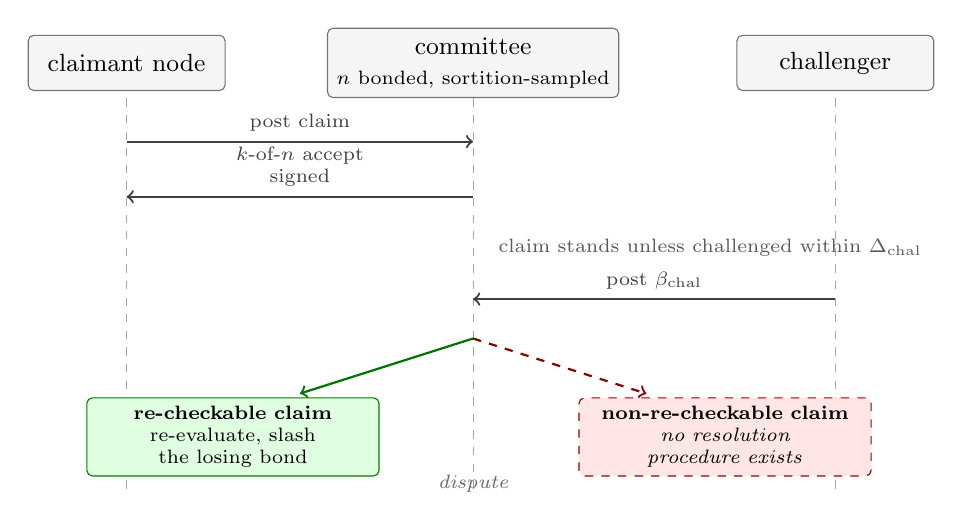
\begin{tikzpicture}[font=\small,
  life/.style={draw=black!55, fill=black!4, rounded corners=2pt, minimum width=2.5cm,
               minimum height=7mm, align=center, font=\small},
  msg/.style={->, thick, black!75},
  ok/.style={draw=green!50!black, fill=green!12, rounded corners=2pt, align=center,
             font=\scriptsize, inner sep=3pt, text width=3.5cm},
  open/.style={draw=red!60!black, fill=red!10, rounded corners=2pt, align=center,
               font=\scriptsize, inner sep=3pt, text width=3.5cm, dashed},
]
\node[life] (cl) at (0,0)  {claimant node};
\node[life] (cm) at (4.4,0) {committee\\{\scriptsize $n$ bonded, sortition-sampled}};
\node[life] (ch) at (9.0,0) {challenger};
\foreach \x in {0,4.4,9.0} \draw[black!35, dashed] (\x,-0.45) -- (\x,-5.5);

\draw[msg] (0,-1.0) -- node[above, font=\scriptsize] {post claim} (4.4,-1.0);
\draw[msg] (4.4,-1.7) -- node[above, font=\scriptsize, align=center]
  {$k$-of-$n$ accept\\{\scriptsize signed}} (0,-1.7);
\node[font=\scriptsize, text=black!65, anchor=west] at (4.6,-2.35)
  {claim stands unless challenged within $\Delta_{\mathrm{chal}}$};
\draw[msg] (9.0,-3.0) -- node[above, font=\scriptsize] {post $\beta_{\mathrm{chal}}$} (4.4,-3.0);

% divergence
\draw[->, thick, green!45!black] (4.4,-3.5) -- ++(-2.2,-0.7);
\draw[->, thick, red!55!black, dashed] (4.4,-3.5) -- ++(2.2,-0.7);
\node[ok]   at (1.35,-4.75) {\textbf{re-checkable claim}\\re-evaluate, slash the losing bond};
\node[open] at (7.6,-4.75) {\textbf{non-re-checkable claim}\\\textit{no resolution procedure exists}};
\node[font=\scriptsize\itshape, text=black!60] at (4.4,-5.35) {dispute};
\end{tikzpicture}
\caption{The bonded-network challenge protocol, showing where the mechanism's soundness depends on
the claim class.}
\label{fig:challenge-protocol}
\end{figure}
%% Drafting note, not prose: the figure must make the divergence between re-checkable and non-re-checkable claim
%% resolution visually explicit, since that divergence is Open Problem~\ref{op:claim-classes}, not a
%% detail.

%% Drain this section's float queue before the next begins.
\FloatBarrier
